\begin{center}
	
\includegraphics[width=\linewidth]{images/unity_okno_belka.png}
\end{center}

W Ubuntu elementy sterujące okna (przyciski zamykania, minimalizacji i maksymalizacji) znajdują się po lewej stronie. Również tytuł okna znajduje się nie na środku, a jest przesunięty ku lewej.

\subsubsection{Elementy sterujące oknami}
\begin{description}
\item[
\includegraphics{images/unity_okno_exit.png}] Zamknij okno.
\item[
\includegraphics{images/unity_okno_min.png}] Minimalizuj okno do paska Launchera.
\item[
\includegraphics{images/unity_okno_max.png}] Maksymalizuj okno do rozmiaru pulpitu. Belka okna, zawierająca opisywane przyciski oraz tytuł, zostanie zintegrowana z panelem menu.
\end{description}

\subsubsection{Przenoszenie i zmiana rozmiaru okna}
Po kliknięciu lewym przyciskiem myszy belki tytułowej okna i przytrzymaniu, możemy je przenieść w dowolne miejsce na pulpicie. Okno można również przenieść przytrzymując przycisk \keys{Alt} --- wówczas wystarczy kliknąć lewym przyciskiem myszy i przytrzymać w dowolnym miejscu okna, które chcemy przenieść.

Aby zmienić rozmiar okna, kursor myszy należy umieścić nad wybraną krawędzią lub rogiem okna. Domyślny kursor zmieni się wówczas w dwustronną strzałkę, zwaną kursorem rozszerzania. Przytrzymanie przycisku myszy, gdy aktywny jest kursor rozszerzania, pozwoli na zmianę rozmiaru i~kształtu okna.

\subsubsection{Przełączanie pomiędzy otwartymi oknami}
W Ubuntu jest wiele sposobów na przełączanie pomiędzy otwartymi programami. Można wykorzystać mysz i kliknąć w dowolnym miejscu otwartych okien. Można wykorzystać ikony otwartych okien na pasku Launchera. Można również wykorzystać kombinację klawiszy \keys{Alt + Tab}.

Gdy mamy otwarte wiele okien, przytrzymanie przycisku \keys{Alt} i wielokrotne naciskanie przycisku \keys{Tab} pozwala wybrać, które okno chcemy aktywować. Domyślnie przełączane w ten sposób są tylko okna z aktywnego obszaru roboczego. Korzystając z kombinacji \keys{Super + Tab} możemy przełączać pomiędzy kolejnymi ikonami na pasku Launchera.

\subsubsection{Ukrywanie wszystkich okien --- pokaż pulpit}
\begin{wrapfigure}{l}{0.05\textwidth}
	\vspace{-10pt}	
	
\includegraphics[width=\linewidth]{images/ikony_pokaz_pulpit.png}
\end{wrapfigure}

Aby ukryć wszystkie okna, nie trzeba ich, jedno po drugim, minimalizować. Można skorzystać ze skrótu \keys{Ctrl + Super + d}. Jego użycie spowoduje ukrycie wszystkich otwartych okien. Ponowne zastosowanie tego skrótu przywróci otwarte okna.

W Ubuntu można również aktywować ikonę \textcolor{ubuntu_orange}{Pokaż pulpit}. Aby to zrobić, kliknij ikonę systemową 
\includegraphics{images/ikony_zasilanie.png} na panelu menu (w prawym górnym rogu) i wybierz \menu{{Ustawienia systemu}>{Osobiste}>{Wygląd}>{Zachowanie}>{Umieść ikonę ,,Pokaż pulpit'' na pasku Launchera}}.

\subsubsection{Przenoszenie otwartych okien pomiędzy obszarami roboczymi}
Przenoszenie otwartych okien pomiędzy obszarami roboczymi jest również dość proste i intuicyjne. Wystarczy uruchomić podgląd obszarów roboczych i przeciągnąć otwarte okno z jednego do drugiego.

\begin{center}
	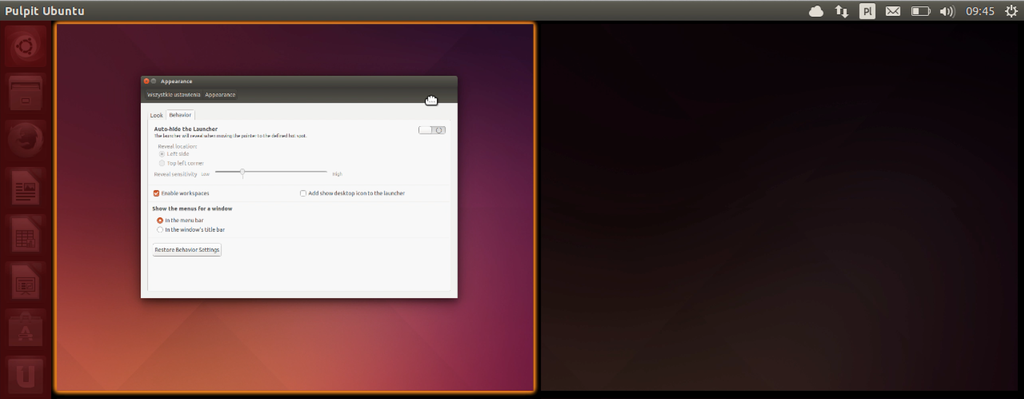
\includegraphics[width=\linewidth]{images/unity_okno_przenoszenie1.png}
\end{center}
\vspace{0.2cm}
\begin{center}
	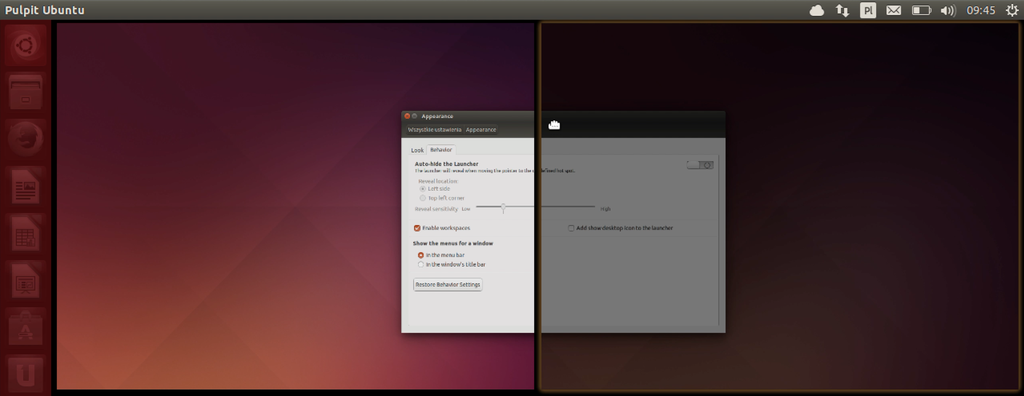
\includegraphics[width=\linewidth]{images/unity_okno_przenoszenie2.png}
\end{center}
\vspace{0.2cm}
\begin{center}
	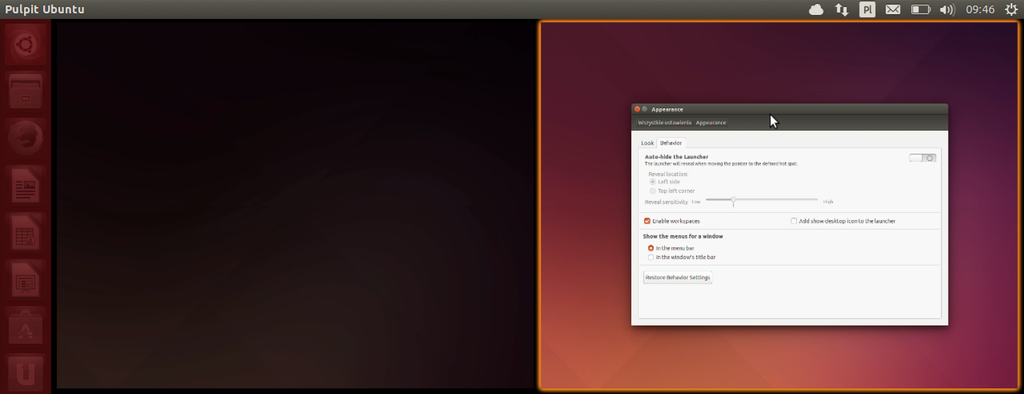
\includegraphics[width=\linewidth]{images/unity_okno_przenoszenie3.png}
\end{center}
\clearpage
Aby przenieść okno do innego obszaru roboczego, można również kliknąć belkę tytułową otwartego okna prawym przyciskiem myszy i z menu kontekstowego wybrać którąś z opcji:
\begin{itemize}
\item \textcolor{ubuntu_orange}{Przenieś do lewego obszaru}, gdy chcemy przenieść okno do lewego obszaru.
\item \textcolor{ubuntu_orange}{Przenieś do prawego obszaru}, gdy chcemy przenieść okno do prawego obszaru.
\item \textcolor{ubuntu_orange}{Przenieś do dolnego obszaru}, gdy chcemy przenieść okno do dolnego obszaru.
\item \textcolor{ubuntu_orange}{Przenieś do górnego obszaru}, gdy chcemy przenieść okno do górnego obszaru.
\item \textcolor{ubuntu_orange}{Przenieś do innego obszaru}, gdy chcemy wybrać do którego konkretnie obszaru ma zostać przeniesione okno.
\end{itemize}

\subsubsection{Zawsze na wierzchu}
Niekiedy okno jakieś aplikacji chcemy mieć zawsze widoczne na pierwszym planie, pomimo tego, że aktualnie pracujemy w innym oknie. Aby utrzymać okno zawsze widoczne na pierwszym planie, należy kliknąć belkę tytułową okna prawym przyciskiem myszy i z menu kontekstowego wybrać opcję \textcolor{ubuntu_orange}{Zawsze na wierzchu}.

\subsubsection{Zawsze na widocznym obszarze roboczym}
W Ubuntu dostępna jest jeszcze jedna bardzo przydatna funkcja, związana z zachowaniem okien. Gdy wykorzystujemy obszary robocze, czasem chcemy, by okno aplikacji zawsze pojawiało się na tym obszarze roboczym, który jest używany. W tym celu należy kliknąć belkę tytułową okna prawym przyciskiem myszy i z menu kontekstowego wybrać opcję \textcolor{ubuntu_orange}{Zawsze na widocznym obszarze roboczym}.
